\documentclass[tikz, border=4pt]{standalone}
\usepackage{tikz}
\usetikzlibrary{arrows.meta}
\begin{document}
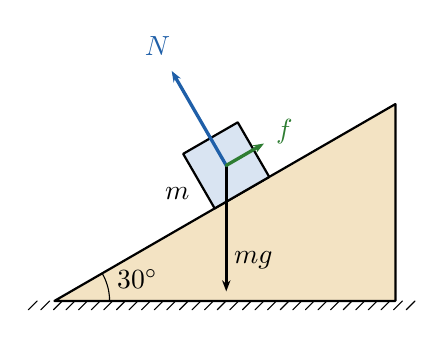
\begin{tikzpicture}[x=1cm, y=1cm]
  \definecolor{tdc1}{HTML}{F3E3C3}
  \definecolor{tdc2}{HTML}{D9E4F2}
  \definecolor{tdc3}{HTML}{1F5FA8}
  \definecolor{tdc4}{HTML}{2E7D32}

  % physics: Mechanics (DiagramTeX)
  \begin{scope}[shift={(0.39,-3.51)}, line cap=round, line join=round]
  \filldraw[fill=tdc1, draw=black, line width=0.8pt] (0,0) -- (4.33,0) -- (4.33,2.5) -- cycle;
  \draw[line width=0.4pt] (-0.22,0) -- (-0.333,-0.113);
  \draw[line width=0.4pt] (-0.06,0) -- (-0.173,-0.113);
  \draw[line width=0.4pt] (0.1,0) -- (-0.013,-0.113);
  \draw[line width=0.4pt] (0.26,0) -- (0.147,-0.113);
  \draw[line width=0.4pt] (0.42,0) -- (0.307,-0.113);
  \draw[line width=0.4pt] (0.58,0) -- (0.467,-0.113);
  \draw[line width=0.4pt] (0.74,0) -- (0.627,-0.113);
  \draw[line width=0.4pt] (0.9,0) -- (0.787,-0.113);
  \draw[line width=0.4pt] (1.06,0) -- (0.947,-0.113);
  \draw[line width=0.4pt] (1.22,0) -- (1.107,-0.113);
  \draw[line width=0.4pt] (1.38,0) -- (1.267,-0.113);
  \draw[line width=0.4pt] (1.54,0) -- (1.427,-0.113);
  \draw[line width=0.4pt] (1.7,0) -- (1.587,-0.113);
  \draw[line width=0.4pt] (1.86,0) -- (1.747,-0.113);
  \draw[line width=0.4pt] (2.02,0) -- (1.907,-0.113);
  \draw[line width=0.4pt] (2.18,0) -- (2.067,-0.113);
  \draw[line width=0.4pt] (2.34,0) -- (2.227,-0.113);
  \draw[line width=0.4pt] (2.5,0) -- (2.387,-0.113);
  \draw[line width=0.4pt] (2.66,0) -- (2.547,-0.113);
  \draw[line width=0.4pt] (2.82,0) -- (2.707,-0.113);
  \draw[line width=0.4pt] (2.98,0) -- (2.867,-0.113);
  \draw[line width=0.4pt] (3.14,0) -- (3.027,-0.113);
  \draw[line width=0.4pt] (3.3,0) -- (3.187,-0.113);
  \draw[line width=0.4pt] (3.46,0) -- (3.347,-0.113);
  \draw[line width=0.4pt] (3.62,0) -- (3.507,-0.113);
  \draw[line width=0.4pt] (3.78,0) -- (3.667,-0.113);
  \draw[line width=0.4pt] (3.94,0) -- (3.827,-0.113);
  \draw[line width=0.4pt] (4.1,0) -- (3.987,-0.113);
  \draw[line width=0.4pt] (4.26,0) -- (4.147,-0.113);
  \draw[line width=0.4pt] (4.42,0) -- (4.307,-0.113);
  \draw[line width=0.4pt] (4.58,0) -- (4.467,-0.113);
  \draw[line width=0.4pt] (0.7,0) -- (0.699,0.046) -- (0.694,0.091) -- (0.687,0.137) -- (0.676,0.181) -- (0.663,0.225) -- (0.647,0.268) -- (0.628,0.31) -- (0.606,0.35);
  \node at (1.054,0.282) {$30^\circ$};
  \filldraw[fill=tdc2, draw=black, line width=0.8pt] (2.035,1.175) -- (2.728,1.575) -- (2.328,2.268) -- (1.635,1.868) -- cycle;
  \draw[line width=1.2pt, -{Stealth[length=4pt]}] (2.182,1.721) -- (2.182,0.121);
  \draw[tdc3, line width=1.2pt, -{Stealth[length=4pt]}] (2.182,1.721) -- (1.489,2.921);
  \draw[tdc4, line width=1.2pt, -{Stealth[length=4pt]}] (2.182,1.721) -- (2.662,1.999);
  \node at (2.526,0.521) {$mg$};
  \node[text=tdc3] at (1.309,3.233) {$N$};
  \node[text=tdc4] at (2.92,2.148) {$f$};
  \node at (1.561,1.363) {$m$};
  \end{scope}
\end{tikzpicture}
\end{document}
